% coding:utf-8

%----------------------------------------
%FOSADSVB, a LaTeX-Code for a summary of digital signal processing
%Copyright (C) 2015, Mario Felder & Michi Fallegger

%This program is free software; you can redistribute it and/or
%modify it under the terms of the GNU General Public License
%as published by the Free Software Foundation; either version 2
%of the License, or (at your option) any later version.

%This program is distributed in the hope that it will be useful,
%but WITHOUT ANY WARRANTY; without even the implied warranty of
%MERCHANTABILITY or FITNESS FOR A PARTICULAR PURPOSE.  See the
%GNU General Public License for more details.
%----------------------------------------

\chapter{Digitale Signale im Zeitbereich}
\section{Signal-Analyse}
\subsection{Sampling}
Die Sample-Frequenz $f_S$ ist durch die Sample-Periode
$T_S$ gegeben:
\[ f_S = \frac{1}{T_S} \]
Aus dem Signal $x(t)$ wird durch die Abtastung:
\[ x(n\cdot T_S) = x[n]\]
Das Signal $x[n]$ ist kausal wenn:
\[ x[n] = 0 \qquad \textrm{für alle } n < 0 \]

%===============================================================================
\subsection{Grundliegende Signale}
Einheitsimpuls oder Diracimpuls:
\[
	\delta = \left\lbrace \begin{matrix}
		0 & : & n \neq 0 \\
		1 & : & n = 0
	\end{matrix} \right.
\]
Einheitsschritt:
\[
	\sigma[n] \mathrm{\ oder\ } u[n] = \left\lbrace \begin{matrix}
		0 & : & n < 0 \\
		1 & : & n \geq 0
	\end{matrix} \right.
\]
Ein periodisches Signal ist beschrieben durch:
\[ x[n] = x[n + T_0/T_S] \qquad \textrm{mit } T_0/T_S = k \]
Ein periodisches Signal muss eine Periodendauer $T_0$ haben,
welche ein ganzzahliges Vielfaches der Sample-Periode $T_S$ ist. 

\begin{center}
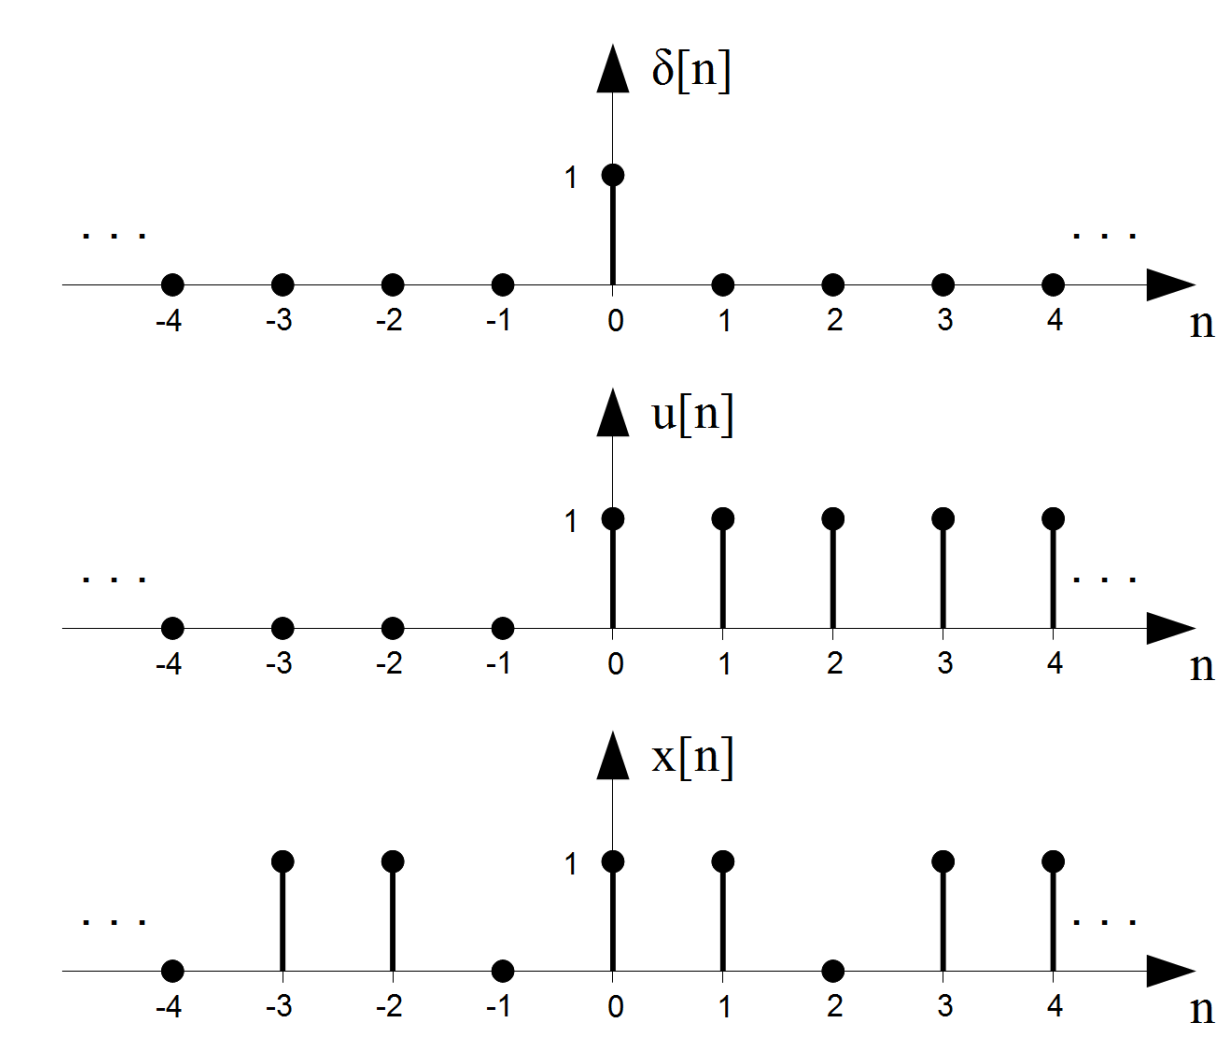
\includegraphics[scale=.7]{../fig/basic_signals}
\end{center}
Komplexe harmonische Sequenz für Fourier-Analyse:
\[ x[n] = \hat{X} \cdot \e^{\im 2 \pi f_0 n T_S} \]
Real- und Imaginäranteil der komplexen Harmonischen:
\[ Re\{\} = \hat{X} \cdot \cos 2 \pi f_0 n T_S \]
\[ Im\{\} = \hat{X} \cdot \sin 2 \pi f_0 n T_S \]

%===============================================================================
\subsection{Statistische Signalparameter}
Observations-Intervall $T$: Der Parameter $N$ entspricht der Anzahl Samples.
\[ T = N \cdot T_S \]
Der Mittelwert (\textbf{mean value}) $\mu_x$ repräsentiert
den DC-Anteil des Signals x[n]:
\[ \mu_x = \frac{1}{N} \sum_{i=0}^{N-1}x[i] \]
Der quadratische Mittelwert (\textbf{quadratic mean value}) ${\rho_x}^2$
korrespondiert zur durchschnittlichen Leistung des Signal $x[n]$
inklusive dem DC-Anteil:
\[ {\rho_x}^2 = \frac{1}{N} \sum_{i=0}^{N-1} x[i]^2 \]
Die \textbf{Varianz} ${\sigma_x}^2$ repräsentiert die durchschnittliche
AC-Leistung des Signals $x[n]$:
\[ {\sigma_x}^2 = \frac{1}{N} \sum_{i=0}^{N-1}(x[i] - \mu_x)^2 \]

%===============================================================================
\subsection{Messverhältnisse und dB}
Leistungsverhältnis (\textbf{power ratio}):
\[ A_{dB} = 10 \cdot \log_{10} \left( \frac{P_1}{P_2} \right) \]
Rauschabstand, Signal-to-noise ratio (\textbf{SNR}):
\[ SNR_{dB} = 10 \cdot \log_{10} \left( \frac{P_{signal}}{P_{noise}} \right) = 20 \cdot \log_{10} \left( \frac{U_{signal}}{U_{noise}} \right) \]
Die Anwendung der Formel mit dem Spannungsverhältnis gilt nur bei Messung über der gleichen Impedanz!\\\\
Matlab-Befehle für Berechnungen mit Leistungsgrössen:\\ 
\verb|  snr   = 10 * log10(sum(s.^2)/sum(r.^2));| (Anwenden des quadratischen Mittelwertes)\\
\verb|  snrac = 10 * log10(sum((s-mean(s)).^2)/sum((r-mean(r)).^2));| (Anwenden der Varianz)\\\\
Matlab-Befehle für Berechnungen mit Signalgrösse (Spannung \verb|s| und Rauschen \verb|r|):\\ 
\verb|  snr = 20*log10(sqrt(sum(s.^2))/sqrt(sum(r.^2)));|
\begin{table}[ht]
  \centering
  \begin{tabular}{ccc} \toprule
  \textbf{Linear}	& \multicolumn{2}{c}{\textbf{Power ratio [dB]}} \\ 
  $a/b$		& Power		& Voltage	\\ \midrule
  $1/1000$	& $-30$		& $-60$		\\
  $1/100$	& $-20$		& $-40$		\\
  $1/10$	& $-10$		& $-20$		\\
  $1/2$		& $\approx$ $-3$ & $\approx$ $-6$\\
  $1$		& 0			& 0			\\
  $2/1$		& $\approx$ 3 & $\approx$ 6\\
  $10/1$	& 10		& 20		\\
  $100/1$	& 20		& 40		\\  
  $1000/1$	& 30		& 60		\\\bottomrule
  \end{tabular}
\end{table}
\newpage
%===============================================================================
\section{Signal Operationen}
\subsection{Korrelation (correlation)}
\textbf{Statische Korrelation (static correlation):} drückt die Ähnlichkeit zweier Signale $x[n]$ und $y[n]$ der selben Länge $N$ als Skalar aus. Bei ungleicher Länge ist zero-padding erlaubt. 
\[ R = \frac{1}{N} \sum_{i=0}^{N-1} x[i] \cdot y[i] \]
Je ähnlicher sich die Signale sind, desto grösser der Wert von $R$.\\\\
\textbf{Lineare Korrelation (linear correlation):}
Falls gilt, dass $x[n] = y[n]$, spricht man von einer Autokorrelation (entspricht dem quadratischen Mittelwert und somit der durchschnittlichen Leistung), sonst auch von einer Kreuzkorrelation.
\[ r_{xy}[n] = \sum_{i=-\infty}^{\infty} x[i] \cdot y[i+n] \]
Die Korrelation ist nicht kommutativ, d.h. $r_{xy}[n] \neq r_{yx}[n]$.\\\\
Resultierende Länge von $r_{xy}$ ($N_{xy}$) und Definitionsbereich:
\[ N_{xy} = N_x + N_y - 1 \hspace{30mm} r_{xy}[n] \neq 0 \mathrm{\ gilt\ für\ } \{ -N_x + 1 \leq n \leq N_y -1 \} \]
Matlab-Befehl für Kreuz- und Autokorrelation: \verb|xcorr()|

\subsection{Faltung (convolution)}
Die Faltung ist der Korrelation ähnlich, das verzögerte Signal wird jedoch an der Y-Achse ($n=0$) gespiegelt. Definition:
\[ z[n] = \sum_{i=-\infty}^{\infty} x[i] \cdot y[-i+n] \]
Die Faltung ist kommutativ:
\[ z[n] = x[n] * y[n] = y[n] * x[n] \]
Resultierende Länge für $z[n]$ ($N_{z}$) und Definitionsbereich:
\[ N_z = N_x + N_y -1 \hspace{30mm} z[n] \neq 0 \mathrm{\ gilt\ für\ } \{ 0 \leq n \leq N_x + N_y -2 \} \]
Beispiel einer Faltung mittels Polonyommultiplikation zweier Signale $x[i]=\{1,1,1,-1\}$ und $y[i]=\{1,1,0.5,0.5\}$:
\begin{flushleft}
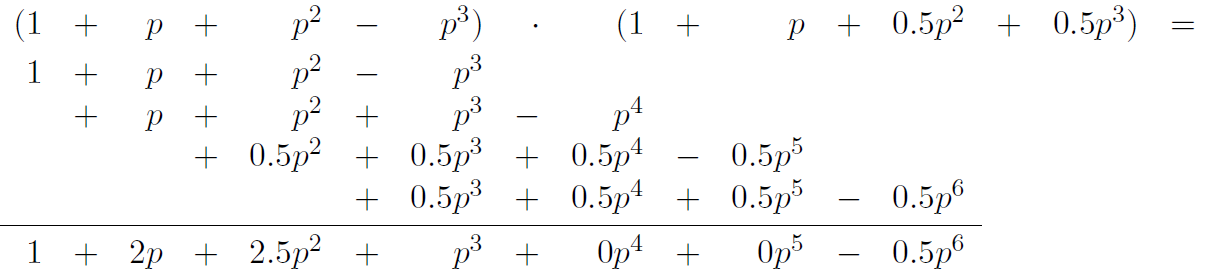
\includegraphics[width=.7\textwidth]{../fig/convolution_example}
\end{flushleft}
Bei der zyklischen Faltung (\textbf{circular convolution}) müssen die beiden
Signale die selbe Länge $N$ haben, oder vorab mit zero-padding auf die selbe Länge $N=N_x+N_y-1$ gebracht werden:
\[ z[n] = x[n] \circledast_N y[n] = y[n] \circledast_N x[n] \]
Lösung durch Matrix:
\[
	\begin{bmatrix}
		y[N]	& y[N-1]	& \ldots & y[0] \\
		y[0]	& y[N]		& \ddots & y[1] \\
		\ddots	& \ddots	& \ddots & \ddots \\
		y[N-1]	& y[N-2]	& \ldots & y[N]
	\end{bmatrix} \cdot \begin{bmatrix}
		x[0] \\ x[1] \\ \vdots \\ x[N]
	\end{bmatrix} = \begin{bmatrix}
		z[0] \\ z[1] \\ \vdots \\ z[N]
	\end{bmatrix}
\]
~\\
Matlabefehl für Faltung: \verb|conv()|\\
Matlabefehl für zyklische Faltung: \verb|convmtx()|
